\documentclass[12pt,a4paper]{article}

\usepackage{amsmath}
\usepackage[dutch]{babel}
\usepackage{hyperref}
\usepackage{enumerate}
\usepackage{graphicx}

\title{Een fysisch systeem voor de computer}
\date{\today}
\author{Derk Rouwhorst en Harmen Stoppels}

\begin{document}
	\begin{titlepage}
	\maketitle
	\end{titlepage}

	\tableofcontents
	\newpage

	\section{Inleiding}
	Wij hebben er voor gekozen om een fysisch systeem te maken voor de computer. Met dit fysisch systeem kunnen tweedimensionale botsingen gesimuleerd worden. Onze hoofdvraag hierbij is:

	Hoe maken we een fysisch systeem dat tweedimensionale botsingen kan simuleren?
	\\Daarbij hebben we de volgende deelvragen bedacht:

	\begin{tabular}{l l}
	\\1.&Hoe werken botsingen bij poolballen?
	\\2.&Met welke natuurkundige en wiskundige formules is de beweging te beschrijven?
	\\3.&Hoe programmeer je deze formules?
	\\4.&Hoe optimaliseer je de snelheid van het programma?
	\end{tabular}

	\newpage
	
	\section{Vectoren}
	We drukken in ons hele profielwerkstuk snelheden, posities en krachten uit in vectoren. Hiermee maken we het rekenwerk een stuk makkelijker en kunnen we formules veel korter opschrijven. We maken gebruik van tweedimensionale vectoren, die uit een $x$- en een $y$-component in het cartesisch co\"{o}rdinatenstelsel bestaan. In de voorbeelden en definities in dit onderdeel gebruiken we ook alleen tweedimensionale vectoren, ook al gelden veel ervan ook voor $n$-dimensionale vectoren.
	
	\subsection{Notatie}
	De namen van vectoren schrijven we dikgedrukt en de componenten boven elkaar met ronde haken eromheen. Een voorbeeld hiervan is $\mathbf{v} = \begin{pmatrix} v_1 \\ v_2 \end{pmatrix} = \begin{pmatrix} 5 \\ -3 \end{pmatrix}$. Dit stelt een vector voor die $5$ naar rechts is gericht en $3$ naar onder.
	
	\subsection{Norm van een vector}
	De norm van een vector is de lengte of grootte. Deze wordt aangeduid met een dubbele verticale streep rondom de vector. Oftewel, de norm van vector $\mathbf{v}$ is $\|\mathbf{v}\| = \sqrt{\left({v_1}^2+{v_2}^2\right)}$
	
	\subsection{Het inwendig product}
	Het inwendig product van twee vectoren is de som van alle componenten met elkaar vermenigvuldigd. Een voorbeeld hiervan is:
	
	\begin{equation*}
		\begin{aligned}
			\mathbf{v} &= \begin{pmatrix} 5 \\ -3 \end{pmatrix}, \mathbf{u} = \begin{pmatrix} 4 \\ 2 \end{pmatrix} \\
			\mathbf{v} \cdot \mathbf{u} &= 5 \times 4 -3 \times 2 = 14\\
		\end{aligned}
	\end{equation*}
	
	Het resultaat van die vermenigvuldiging en optelling is het best te zien als hoeveel de kortste vector van de twee in het domein van de langste zit. Deze eigenschap is handig te gebruiken bij het kijken of twee bewegende cirkels elkaar op een bepaald tijdsinterval raken.
	
	Het bewijs voor deze eigenschap maakt gebruik van de cosinusregel. Gegeven de vectoren $\mathbf{u}=\begin{pmatrix} u_1 \\ u_2 \end{pmatrix}$ en $\mathbf{v}=\begin{pmatrix} v_1 \\ v_2 \end{pmatrix}$ met hetzelfde beginpunt en een onderlinge hoek $\gamma$ en vector $\mathbf{c}$ tussen beide uiteinden van de vectoren, geldt er:
 	\begin{equation}
		\begin{aligned}
			\|\mathbf{c}\|^2 = \left\{ 
				\begin{array}{l l}
 	 				\sqrt{(a_1-b_1)^2+(a_2-b_2)^2} \\
  					{\|\mathbf{a}\|}^2 + {\|\mathbf{b}\|}^2 - 2 \cdot \|\mathbf{a}\| \cdot \|\mathbf{b}\| \cdot \cos\gamma 
 	 			\end{array} 
 	 		\right.
		\end{aligned}
	\end{equation}
	\\Hieruit volgt:
	\begin{equation}
		\label{inproduct-cosinus}
		\begin{aligned}
			(a_1-b_1)^2 + (a_2-b_2)^2 &= {\|\mathbf{a}\|}^2 + {\|\mathbf{b}\|}^2 - 2 \cdot {\|\mathbf{a}\|} \cdot {\|\mathbf{b}\|} \cdot \cos\gamma \\
			{a_1}^2 + {a_2}^2+ {b_1}^2 + {b_2}^2 - 2a_1b_1 - 2a_2b_2 &= {a_1}^2 + {a_2}^2+ {b_1}^2 + {b_2}^2 - 2 \cdot {\|\mathbf{a}\|} \cdot {\|\mathbf{b}\|} \cdot \cos\gamma \\
			-2a_1b_1 - 2a_2b_2 &= - 2 \cdot {\|\mathbf{a}\|} \cdot {\|\mathbf{b}\|} \cdot \cos\gamma \\
			-2(a_1b_1 + a_2b_2) &= - 2 \cdot {\|\mathbf{a}\|} \cdot {\|\mathbf{b}\|} \cdot \cos\gamma \\
			-2(\mathbf{a} \cdot \mathbf{b}) &= - 2 \cdot \|\mathbf{a}\| \cdot \|\mathbf{b}\| \cdot \cos\gamma \\
			\mathbf{a} \cdot \mathbf{b} &= \|\mathbf{a}\| \cdot \|\mathbf{b}\| \cdot \cos\gamma\\
		\end{aligned}
	\end{equation}

	Met het resultaat hiervan kunnen we later geometrische berekeningen doen, zonder de voor de computer ``tijdrovende'' functie cosinus of sinus te gebruiken.
	
	\subsection{Eenheidsvector}
	Een eenheidsvector is een vector waarvan de lengte 1 is. Het handige van zo'n vector is dat hij, vermenigvuldigd met een getal, zijn richting behoudt en de lengte van dat getal aanneemt. Stel, je hebt de richting waarin een voorwerp beweegt als eenheidsvector, dan geeft vermenigvuldiging met de snelheid, de snelheid als vector. De notatie van een eenheidsvector wordt gedaan met een dakje erop: $\|\mathbf{\hat{a}}\| = 1$.

	\newpage	

	\section{Tijdstippen van botsingen}
	
	\subsection{Cirkel tegen cirkel}
	Kijken of twee cirkels elkaar raken is theoretisch erg makkelijk te doen. Het komt er simpelweg op neer dat de cirkels elkaar raken als de som van de stralen groter of gelijk is aan de afstand tussen de middelpunten. Het wordt echter lastiger als de cirkels snel bewegen en elkaar tussen twee frames raken. Het probleem is dat het gros van de botsingen tussen cirkels juist tussen twee frames gebeurt.
	
	\subsubsection{Formule}
	\begin{figure}[h]
		\centerline{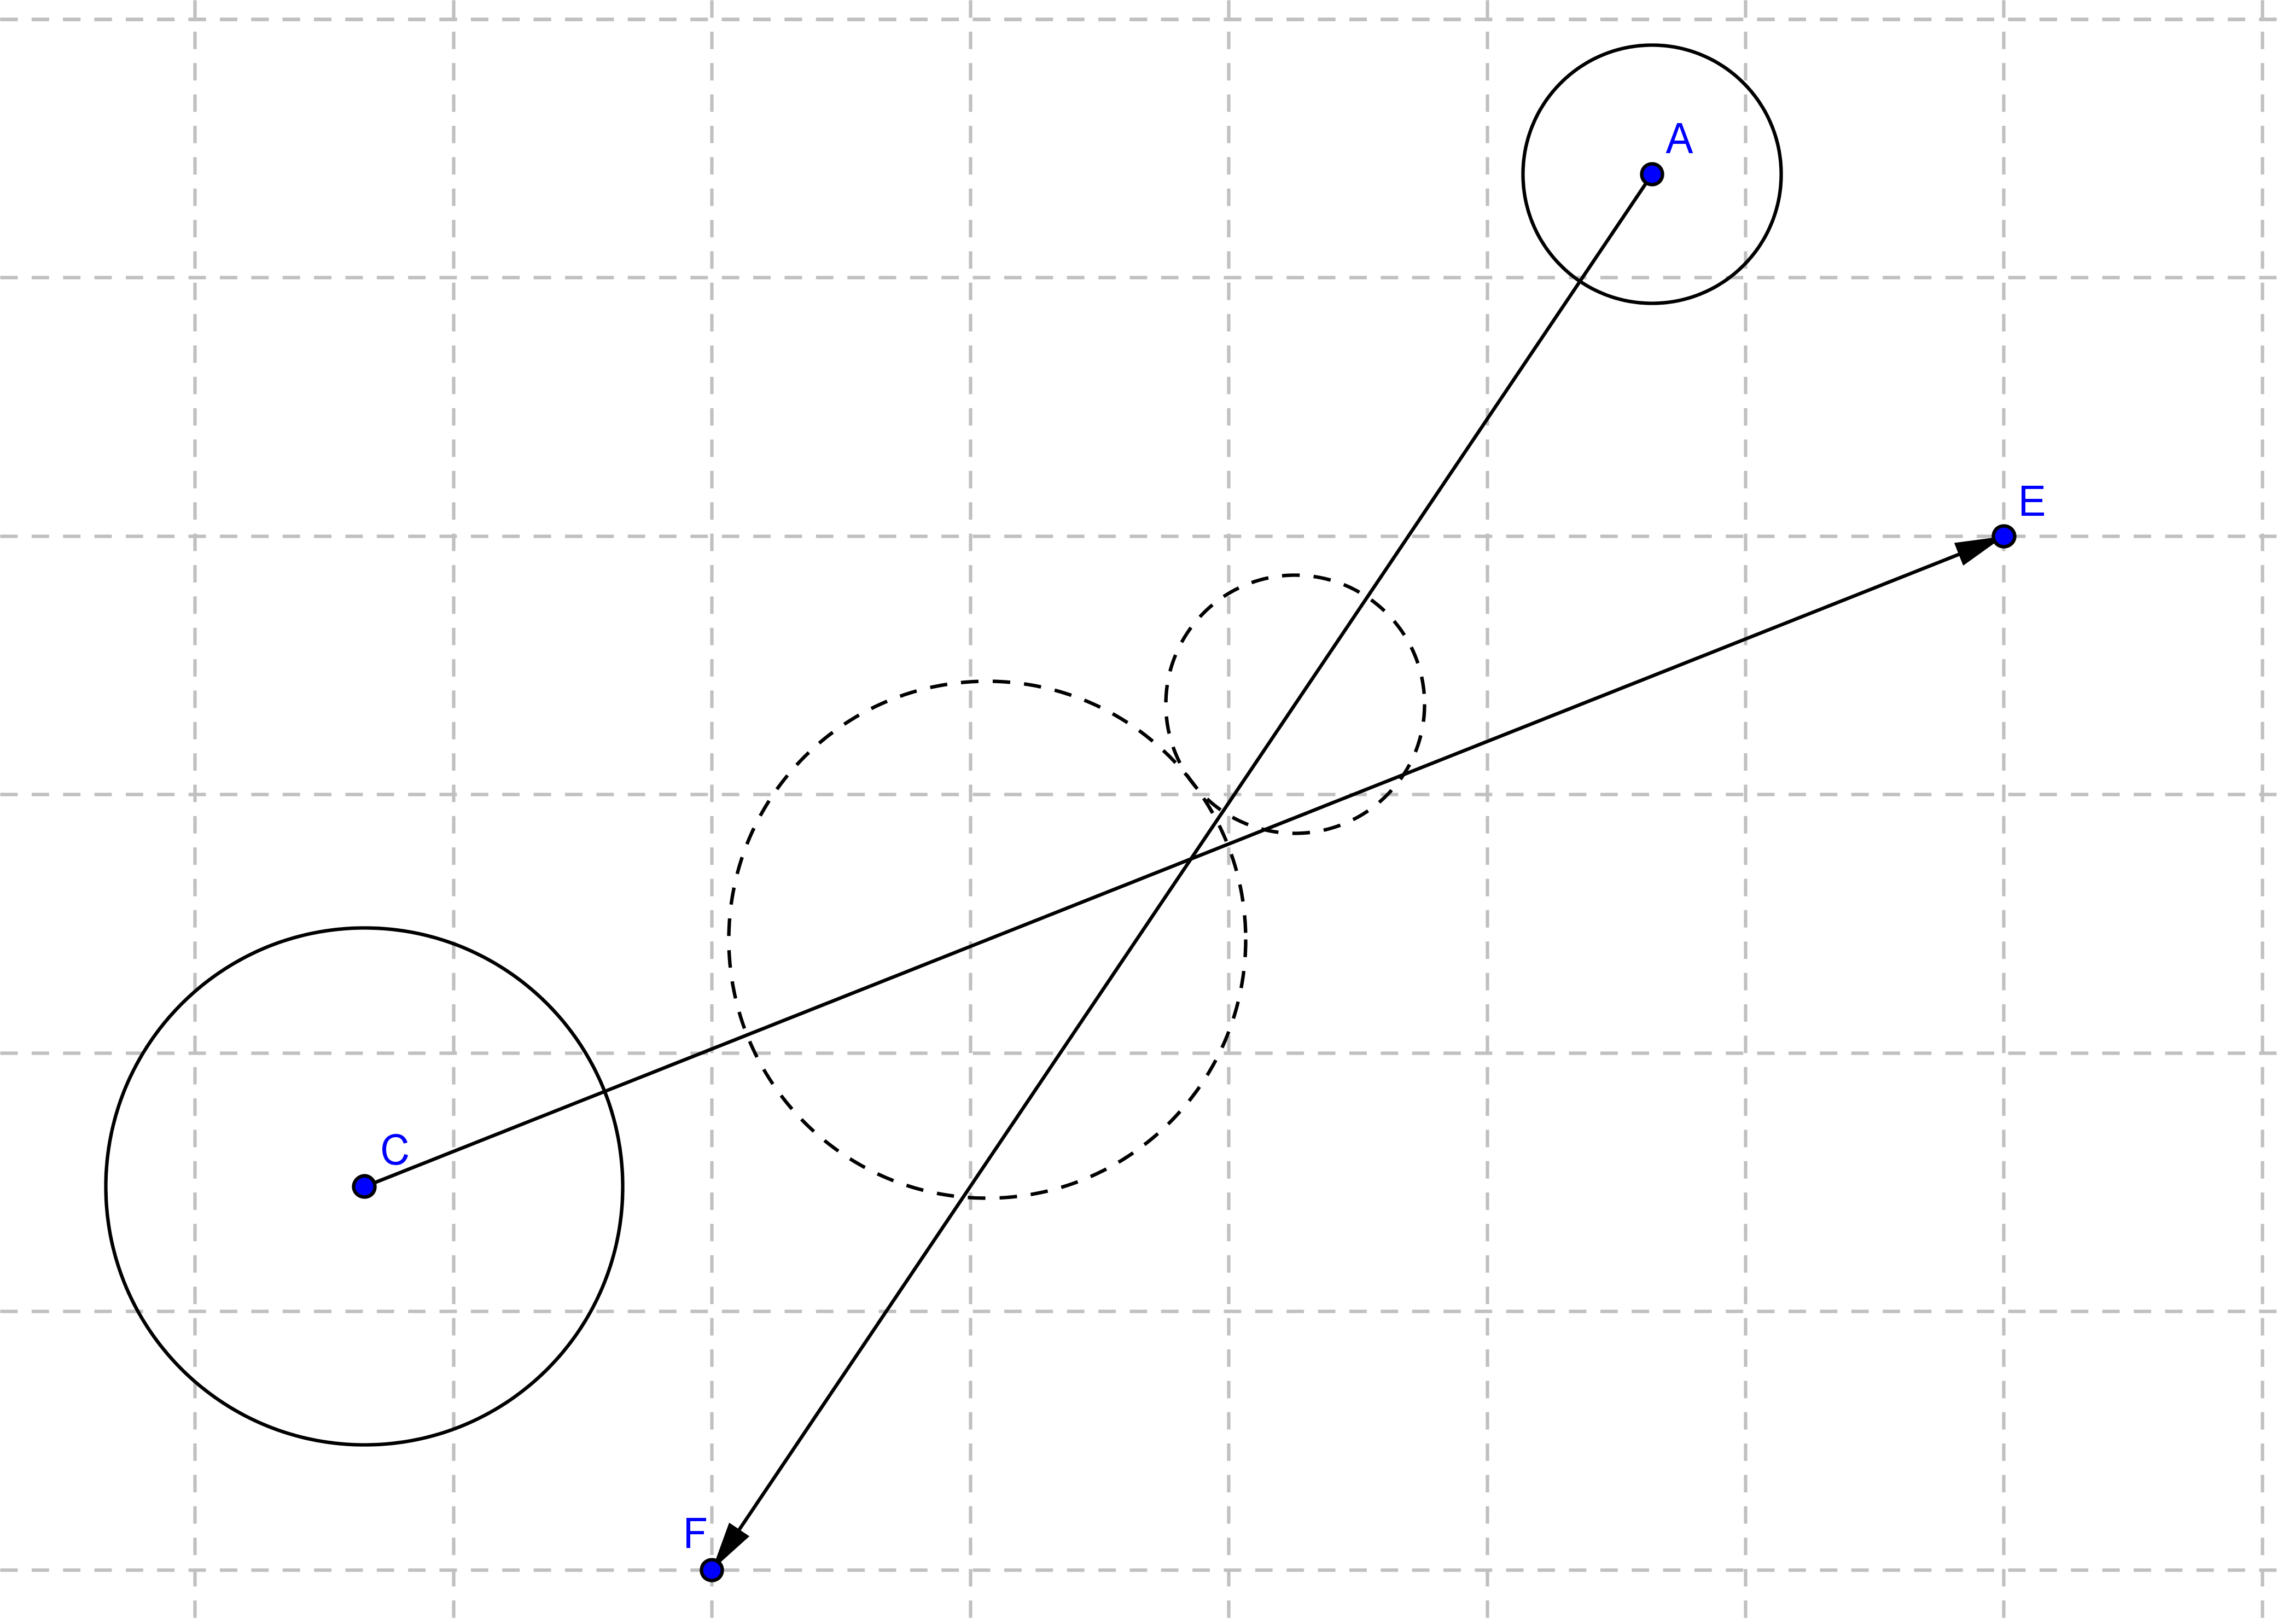
\includegraphics[width=\textwidth]{Bal-Bal.png}}
		\caption{Botsing tussen twee ballen}
		\label{bal-bal}
	\end{figure}
	
	Bij het berekenen van de nieuwe posities van de ballen in het volgende frame, moeten we dus als eerste kijken of ze ondertussen botsen, als tweede berekenen wanneer dat is en als derde uitvinden wat voor gevolg die botsing heeft.
	
	Om de uiteindelijke vergelijking te versimpelen gaan wij ervan uit dat elk voorwerp tussen twee frames een constante snelheid heeft en over een rechte lijn beweegt. Dit klopt niet met de realiteit, maar omdat de tijd tussen twee frames erg klein is, maakt het niet zo veel uit.
	
	De cirkels kunnen elkaar op het tijdsinterval tussen twee frames hoogstens twee keer raken (als je geen rekening houdt met het effect van de botsing), namelijk wanneer ze voor het eerst tegen elkaar aankomen en wanneer ze door elkaar heen zijn gevlogen. De botsing die wij moeten vinden is de eerste, de tweede vindt natuurlijk nooit plaats.
	
	Allereerst noemen we de tijd in het eerste frame $t=0$ en in het tweede frame $t=1$. We zoeken een waarde van $t$ waarvoor geldt dat $0 \le t < 1$ en waarbij de afstand tussen de middelpunten gelijk is aan de som van de stralen.
	
	De posities van de ballen geven we aan met vectoren. De nieuwe positie bestaat uit de oude positie met daarbij opgeteld de snelheidsvector vermenigvuldigd met de tijd. Wat we krijgen is dus:
	\begin{equation}
		\begin{aligned}
			\mathbf{X} &= \mathbf{X} + \mathbf{v}t\\
		\end{aligned}
	\end{equation}
	\\Vul je $t=0$ in, dan krijg je de positie in frame 1; vul je $t=1$, dan krijg je de positie in frame 2 (geen rekening gehouden met het effect van een mogelijke botsing).
	
	We moeten nu een vergelijking opzetten en oplossen voor $t$, waarin we de relatieve afstand tussen twee ballen gelijkstellen aan de som van de stralen:
	
	\begin{equation}
		\begin{aligned}
			 \|\mathbf{X_1} + \mathbf{v_1}t  - \mathbf{X_2} -  \mathbf{v_2}t \| &= r_1 + r_2 \\
			 \|\mathbf{X_{rel}} + \mathbf{v_{rel}}t \| &= r_1 + r_2\\
		\end{aligned}
	\end{equation}
	\\Beide kanten kwadrateren geeft:
	\begin{equation}
		\label{botsing}
		\begin{aligned}
			\mathbf{v_{rel}}^2 t^2 + 2 \mathbf{X_{rel}} \mathbf{v_{rel}} + \mathbf{X_{rel}}^2  &= (r_1 + r_2)^2 \\
			(\mathbf{v_{rel}} \cdot \mathbf{v_{rel}})t^2 + 2(\mathbf{X_{rel}} \cdot \mathbf{v_{rel}})t + \mathbf{X_{rel}} \cdot \mathbf{X_{rel}} &= (r_1 + r_2)^2 \\
			(\mathbf{v_{rel}} \cdot \mathbf{v_{rel}})t^2 + 2(\mathbf{X_{rel}} \cdot \mathbf{v_{rel}})t + \mathbf{X_{rel}} \cdot \mathbf{X_{rel}} - (r_1 + r_2)^2 &= 0\\
		\end{aligned}
	\end{equation}
	\\Deze vergelijking is een eenvoudige vierkantsvergelijking, die ook in een iets alternatieve vorm kan worden geschreven om rekentijd te beperken:
	
	\begin{equation}
		\label{a2bc}
		\begin{aligned}
			at^2+2bt+c &= 0 \\
			t^2+\tfrac{2b}{a}t &= -\frac{c}{a} \\
			\left( t+\tfrac{b}{a} \right)^2 &= \frac{b^2}{a^2} -\frac{c}{a} \\
			t + \tfrac{b}{a} &= \pm \sqrt{\frac{b^2 - ac}{a^2}} \\
			t &= \frac{-b \pm \sqrt{b^2 - ac}}{a}\\
		\end{aligned}
	\end{equation}
	\\Vergelijking \eqref{a2bc} kunnen we nu toepassen op vergelijking \eqref{botsing}:
	
	\begin{equation}
		\begin{aligned}
			a &= \mathbf{v_{rel}} \cdot \mathbf{v_{rel}} \\
			b &= \mathbf{X_{rel}} \cdot \mathbf{v_{rel}} \\
			c &= \mathbf{X_{rel}} \cdot \mathbf{X_{rel}} - (r_1 + r_2)^2\\
		\end{aligned}
	\end{equation}
	
	\subsubsection{Simulatie}
	We hebben deze formule omgezet naar een simulatie in \href{http://www.geogebra.org/webstart/geogebra.html}{Geogebra}, om te kijken of de formule klopte; zie de bijlage met de bestandsnaam Bal-Bal.ggb. Zowel de verplaatsingsvectoren, beginposities en de stralen van beide cirkels zijn aan te passen, en als er binnen het begin- en eindpunt een botsing is, worden de cirkels opnieuw gestippeld getekend op de plaats van de botsing.
	
	\subsection{Cirkel tegen lijnstuk}
	Om erachter te komen of een cirkel een lijnstuk raakt binnen een tijdinterval, gebruiken we een formule die het punt op het lijnsegment geeft dat het dichtst bij het midden van de cirkel ligt.
	
	\subsubsection{Tijdstippen van botsingen}
	Gegeven is een lijnstuk $AB$ en een cirkel die met constante snelheid over lijnstuk $CD$ beweegt. De cirkel heeft straal $r$ en botst tijdens zijn beweging misschien tegen lijnstuk $AB$. Op tijdstip $t=0$ bevindt het middelpunt van de cirkel zich op $C$, op tijdstip $t=1$ bevindt het zich op $D$. We zoeken dus naar de eerste waarde voor $t$ tussen $0$ en $1$ waarop de cirkel lijnstuk $AB$ raakt.
	
	Om dit probleem op te lossen gebruiken een vergelijking voor de afstand van een punt tot een lijn, en die afstand moet gelijk zijn aan de straal van de cirkel. Als $AB$ en $CD$ niet parallel lopen, krijgen we twee oplossingen voor onze vergelijking. De eerste is de botsing, de tweede oplossing geeft het tijdstip aan waarop de cirkel door $AB$ is gevlogen en het lijnstuk dan raakt.
	
	\begin{figure}[h]
		\centerline{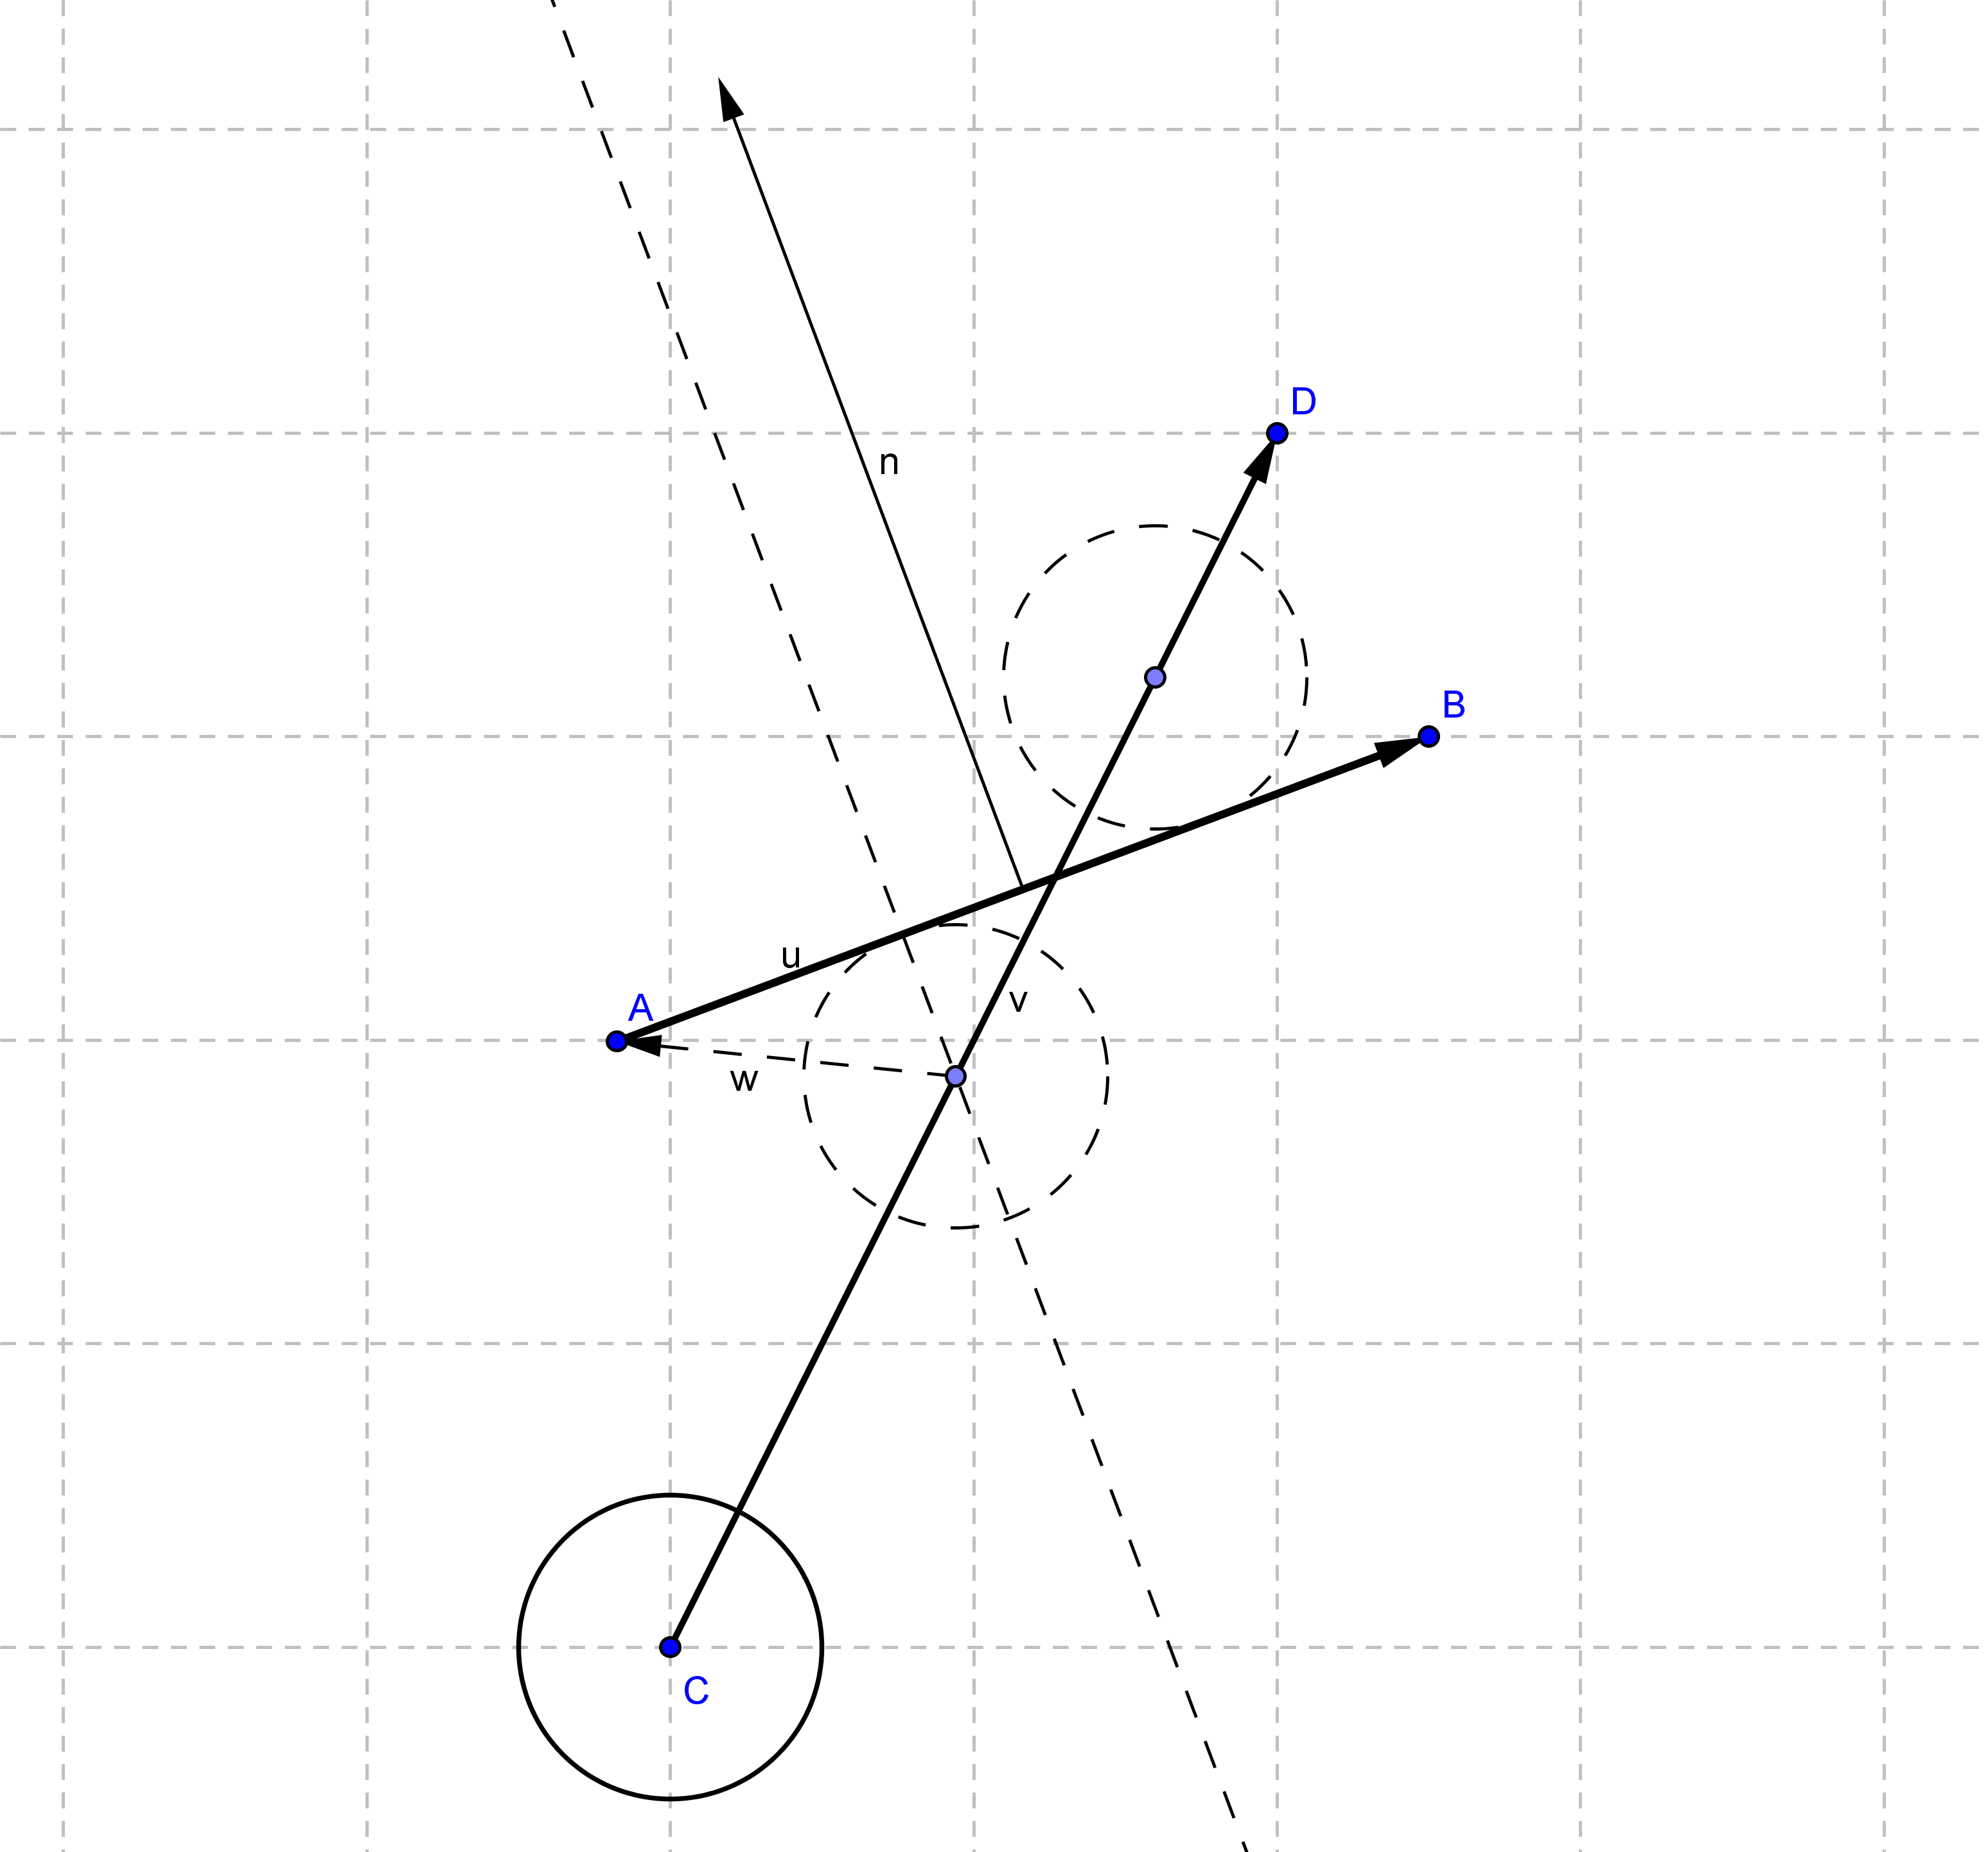
\includegraphics[width=\textwidth]{Bal-Lijn.png}}
		\caption{Botsing tussen een bal en een lijnstuk}
		\label{bal-lijn}
	\end{figure}
	
	Eerst defini\"{e}ren we $\mathbf{n}$ als de normaalvector van $AB$. Daarna vinden we de afstand van een punt tot een lijnstuk door middel van de eigenschappen van het inproduct van twee vectoren:
	\begin{equation}
		\label{eigenschappeninproduct}
		cos \gamma = \frac{|\mathbf{w} \cdot \mathbf{n}|}{\| \mathbf{w} \| \| \mathbf{n} \|}
	\end{equation}
	Verder geldt in het driehoekje met zijden $\mathbf{w}$ en $r$:
	\begin{equation}
		\label{driehoekmetzijdew}
		cos \gamma = \frac{r}{\| \mathbf{w}\| }
	\end{equation}
	Samenvoeging van \eqref{eigenschappeninproduct} en \eqref{driehoekmetzijdew} geeft:
	\begin{equation}
		\label{definitiestraal}
		\begin{aligned}
			\frac{r}{\| \mathbf{w}\| } &= \frac{|\mathbf{w} \cdot \mathbf{n}|}{\| \mathbf{w} \| \| \mathbf{n} \|} \\
			r &= \frac{|\mathbf{w} \cdot \mathbf{n}|}{\| \mathbf{n} \|} \\
			r \, \| \mathbf{n} \| &= |\mathbf{w} \cdot \mathbf{n}| \\
			\pm \, r \, \| \mathbf{n} \| &= \mathbf{w} \cdot \mathbf{n}
		\end{aligned}
	\end{equation}
	Vector $\mathbf{w}$ begint in het middelpunt van de cirkel op $CD$ en gaat naar punt $A$, en is dus als volgt de defini\"{e}ren:
	\begin{equation}
		\label{definitiew}
		\begin{aligned}
			\mathbf{w} &= \mathbf{a} - (\mathbf{c} + t \left(\mathbf{d} - \mathbf{c} \right)) \qquad 0 \leq t \leq 1 \\
			&= \mathbf{a} - \mathbf{c} - t \left(\mathbf{d} - \mathbf{c} \right)
		\end{aligned}
	\end{equation}
	Als je $t=0$ invult krijg je $\mathbf{w} = \mathbf{a} - \mathbf{c}$ en als je $t=1$ invult krijg je $\mathbf{w} = \mathbf{a} - \mathbf{d}$.
	
	Nu kun je \eqref{definitiew} invullen in \eqref{definitiestraal} en kun je $t$ uitdrukken in andere variabelen:
	\begin{equation}
		\begin{aligned}
			\pm \, r \, \| \mathbf{n} \| &= (\mathbf{a} - \mathbf{c} - t \left(\mathbf{d} - \mathbf{c} \right)) \cdot \mathbf{n} \\
			\pm \, r \, \| \mathbf{n} \| &= (\mathbf{a} - \mathbf{c}) \cdot \mathbf{n} - t \left(\mathbf{d} - \mathbf{c} \right) \cdot \mathbf{n} \\
			t \left(\mathbf{d} - \mathbf{c} \right) \cdot \mathbf{n} &= \pm \, r \, \| \mathbf{n} \| + (\mathbf{a} - \mathbf{c}) \cdot \mathbf{n} \\
			t &= \frac{\pm \, r \, \| \mathbf{n} \| + (\mathbf{a} - \mathbf{c}) \cdot \mathbf{n}}{\left(\mathbf{d} - \mathbf{c} \right) \cdot \mathbf{n}}
		\end{aligned}
	\end{equation}
	
	\subsubsection{Punt op lijnstuk dichtste bij cirkel}
	DIT STUKJE IS NU VERGELIJKBAAR MET HET VORIGE. HET MOET OPNIEUW GESCHREVEN WORDEN.
	
	Omdat we met vectoren werken is het heel makkelijk om te bepalen welk punt op een lijnstuk het dichtst bij het middelpunt van een cirkel ligt. Voor het gemak noemen we de uiteinden van het lijntuk $A$ en $B$, het middelpunt van de cirkel $C$, en we defini\"{e}ren $P$ als het punt op het lijnstuk het dichtste bij $C$. $P$ is dus een loodrechte projectie van $C$ op $AB$. Verder stellen we het lijnstuk voor als een vector $\mathbf{v}$ vanuit punt $A$ en tekenen we een vector $\mathbf{w}$ vanuit $A$ naar $C$. Eerder bleek al dat geldt \eqref{inproduct-cosinus}:
	\begin{equation}
		\label{inproduct-cosinus-toegepast}
		\begin{aligned}
			\mathbf{v} \cdot \mathbf{w} &= \|\mathbf{v}\| \cdot \|\mathbf{w}\| \cdot \cos\gamma \\
			\cos\gamma &= \frac{\mathbf{v} \cdot \mathbf{w}}{\|\mathbf{v}\| \cdot \|\mathbf{w}\|}\\
		\end{aligned}
	\end{equation}
	\\Verder geldt in driehoek $\triangle ACP$, waarbij $AC = \mathbf{w}$:
	\begin{equation}
		\label{cos-gamma}
		\cos\gamma = \frac{AP}{\|\mathbf{w}\|} = \frac{x}{\|\mathbf{w}\|}
	\end{equation}

	We zijn nu op zoek naar de verhouding tussen $x$ en $\mathbf{w}$. Dat geeft een indicatie van hoever punt $P$ op het lijnstuk ligt. Is die verhouding kleiner dan 0, of groter dan 1, dan ligt het punt dat het dichtste bij $C$ ligt, voorbij het lijnstuk. Ligt het ertussen, dan ligt het punt ergens tussen $A$ en $B$.
	Combineer je \eqref{inproduct-cosinus-toegepast} en \eqref{cos-gamma}, dan krijg je:
	\begin{equation}
		\begin{aligned}
		\frac{x}{\|\mathbf{w}\|} &= \frac{\mathbf{v} \cdot \mathbf{w}}{\|\mathbf{v}\| \cdot \|\mathbf{w}\|} \\
		                       x &= \frac{\mathbf{v} \cdot \mathbf{w}}{\|\mathbf{v}\|} \\
		\frac{x}{\|\mathbf{v}\|} &= \frac{\mathbf{v} \cdot \mathbf{w}}{\|\mathbf{v}\| \cdot \|\mathbf{v}\|} \\
		\frac{x}{\|\mathbf{v}\|} &= \frac{\mathbf{v} \cdot \mathbf{w}}{\mathbf{v} \cdot \mathbf{v}}\\
		\end{aligned}
	\end{equation}
	\\We hebben dit ook in \href{http://www.geogebra.org/webstart/geogebra.html}{Geogebra} gesimuleerd, zie in de bijlage het bestand Bal-Lijn.ggb. Variabelen zijn hierbij het de positie van het de begin- en eindpunten van het lijnstuk (dat is meteen al vector $\mathbf{v}$ geworden) en de positie van de cirkel.
	
	\newpage

	\section{Theorie van botsingen}
	In de natuurkunde is een botsing elke interactie tussen deeltjes of voorwerpen die dicht genoeg bij elkaar komen om energie uit te wisselen. Bij een botsing tussen twee lichamen (voorwerpen) zullen er van het moment van eerste aanraking af vormveranderingen optreden, waardoor veerkrachten worden opgewekt. Als deze veerkrachten groot genoeg zijn, zullen de lichamen zich na de botsing weer van elkaar verwijderen. In het algemeen zijn de snelheden van beide lichamen voor en na de botsing verschillend, zodat overdracht van kinetische energie (bewegingsenergie) heeft plaatsgevonden.

	\subsection{Elastische botsing}
	Als twee biljartballen met elkaar botsen, treedt er slechts een tijdelijke vormverandering op; aan het eind van de botsing krijgen de ballen hun oude vorm weer terug. Dit heet dan van een volkomen elastische (veerkrachtige) botsing, waarvoor de wet van behoud van bewegingsenergie geldig is.

	\subsection{Onelastische botsing}
	Wordt er bijvoorbeeld een kogel in een zandzak geschoten en blijft de kogel daarin steken, dan bewegen beide lichamen zich als \'{e}\'{e}n geheel verder. Bij deze volkomen onelastische botsing treedt een blijvende vormverandering op, zodat de wet van behoud van bewegingsenergie niet geldig is, omdat een deel van de bewegingsenergie verbruikt is voor deze vervorming.
	Tussen deze twee voorbeelden in liggen gedeeltelijke veerkrachtige botsingen.

	\subsection{De wet van behoud van impuls}
	Omdat voor elke botsing geldt dat de krachten die de lichamen op elkaar uitoefenen, even groot zijn, tegengesteld gericht zijn en even lang werken, is de stoot van de botsingskrachten nul:
	\begin{equation}
		  \int_0^t \sum F_1\,dt = 0\\
	\end{equation}

	De verandering van de impuls van de beide lichamen samen is dus nul, met andere woorden voor elk type botsing geldt de wet van behoud van impuls.
Voor de gevolgen van een botsing is het ook belangrijk hoe de twee lichamen elkaar treffen. Als je aanneemt dat de beide lichamen in \'{e}\'{e}n plat vlak bewegen, dan kunnen de beide snelheidsvectoren samenvallen met de verbindingslijn tussen de beide zwaartepunten. Dit heet een centrale botsing (analoog met een frontale botsing tussen auto's). Maken deze vectoren hoeken met deze verbindingslijn, dan spreekt men van een niet-centrale botsing (bijvoorbeeld een botsing tussen twee auto's op een straathoek).

	\section{Berekening van de snelheden na de botsing}
	In de meeste gevallen zijn de snelheden van de ballen na de botsing, anders dan de snelheden van de ballen voor de botsing. Deze snelheden kunnen berekend worden met behulp van de snelheden v\'{o}\'{o}r de botsing en de massa's van beide ballen. Een eenvoudige botsing is de centrale botsing, ook wel eendimensionale botsing genoemd.

	\subsection{Berekening voor een centrale botsing}
	De snelheden na een botsing bij een centrale botsing kunnen op meerdere manieren berekend worden. Hier volgen twee methodes waarop deze berekend kunnen worden. Bij  de eerste methode gebruiken wordt gebruikt gemaakt van de wet van behoud van energie en de wet van behoud van impuls. Bij de tweede methode wordt alleen de wet van behoud van impuls en de gemeenschappelijke snelheid gebruikt.

	\subsubsection{Met behulp van de wet van behoud van energie en impuls}
	Omdat we te maken hebben met volkomen elastische botsingen geldt de wet van behoud van energie \eqref{energie} en de wet van behoud van impuls \eqref{impuls}. Met deze twee wetten kunnen we de snelheden van de ballen na de botsing berekenen.
	\begin{equation}
		\label{energie}
		\frac{1}{2} m_1 {o_1}^2 + \frac{1}{2} m_2 {o_2}^2 = \frac{1}{2} m_1{v_1}^2 + \frac{1}{2}m_2 {v_2}^2\\
	\end{equation}
	\begin{equation}
		\label{impuls}
		m_1 o_1 + m_2 o_2 =  m_1 v_1 + m_2 v_2\\
	\end{equation}
	\\Waarbij:
	\begin{equation}
		\begin{aligned}
			m_1 &= \text{massa van lichaam 1}\\
			m_2 &= \text{massa van lichaam 2}\\
			o_1 &= \text{snelheid van lichaam 1 voor de botsing}\\
			o_2 &= \text{snelheid van lichaam 2 voor de botsing}\\
			v_1 &= \text{snelheid van lichaam 1 na de botsing}\\
			v_2 &= \text{snelheid van lichaam 2 na de botsing}\\
		\end{aligned}
	\end{equation}

	We hebben nu twee vergelijkingen met twee onbekenden, namelijk $v_1$ en $v_2$. We kunnen $v_2$ uit beide vergelijkingen elimineren, en daarna de vergelijkingen aan elkaar gelijk stellen, zodat we als onbekende alleen $v_1$ over houden.
	\\Als eerste de vergelijking van de wet van behoud van energie:
	\begin{equation}
		\label{energie-{v_1}^2}
		\begin{aligned}
			\frac{1}{2} m_1 {o_1}^2 + \frac{1}{2} m_2 {o_2}^2 &= \frac{1}{2} m_1{v_1}^2 + \frac{1}{2}m_2 {v_2}^2\\
			m_1 {o_1}^2 + m_2 {o_2}^2 &= m_1{v_1}^2 + m_2 {v_2}^2\\
			m_1 {o_1}^2 + m_2 {o_2}^2 - m_2 {v_1}^2 &= m_2{v_2}^2\\
			\frac{m_1 {o_1}^2 + m_2 {o_2}^2 - m_1 {v_1}^2}{m_2} &= {v_2}^2\\
		\end{aligned}
	\end{equation}
	\\Dan de vergelijking van de wet van behoud van impuls:
	\begin{equation}
		\label{impuls-{v_1}^2}
		\begin{aligned}
			m_1 o_1 + m_2 o_2 &=  m_1 v_1 + m_2 v_2\\
			m_1 o_1 + m_2 o_2 - m_1 v_1 &=  m_2 v_2\\
			\frac{m_1 o_1 + m_2 o_2 - m_1 v_1}{m_2} &= v_2\\
			{\left(\frac{m_1 o_1 + m_2 o_2 - m_1 v_1}{m_2}\right)}^2 &= {v_2}^2\\
		\end{aligned}
	\end{equation}
	\\De uitkomsten van \eqref{impuls-{v_1}^2} en \eqref{energie-{v_1}^2} aan elkaar gelijk stellen geeft:
	\begin{equation}
		\begin{aligned}
			&\frac{m_1 {o_1}^2 + m_2 {o_2}^2 - m_1 {v_1}^2}{m_2} = {\left(\frac{m_1 o_1 + m_2 o_2 - m_1 v_1}{m_2}\right)}^2\\
			&= \frac{\left({m_1}^2{o_1}^2 + {m_2}^2{o_2}^2 + {m_1}^2{v_1}^2\right) + \left(2m_1m_2o_1o_2 - 2{m_1}^2o_1v_1 - 2m_1m_2o_2v_1\right)}{{m_2}^2}\\
		\end{aligned}
	\end{equation}
	\\Deze vergelijking oplossen, zodat je een vierkantsvergelijking krijgt:
	\begin{equation}
		\begin{aligned}
			&{m_1}^2{o_1}^2 + {m_2}^2{o_2}^2 + {m_1}^2{v_1}^2 + 2m_1m_2o_1o_2 - 2{m_1}^2o_1v_1 - 2m_1m_2o_2v_1 =\\
			&m_1m_2{o_1}^2 + {m_2}^2{o_2}^2 - m_1m_2{v_1}^2\\
			&{m_1}^2{o_1}^2 + {m_1}^2{v_1}^2 + 2m_1m_2o_1o_2 - 2{m_1}^2o_1v_1 - 2m_1m_2o_2v_1 =\\
			&m_1m_2{o_1}^2 - m_1m_2{v_1}^2\\
			&{m_1}^2{o_1}^2 + {m_1}^2{v_1}^2 + 2m_1m_2o_1o_2 - 2{m_1}^2o_1v_1 - 2m_1m_2o_2v_1 - m_1m_2{o_1}^2 + m_1m_2{v_1}^2 = 0\\
			&\left({m_1}^2+m_1m_2\right){v_1}^2+\left(-2{m_1}^2o_1-2m_1m_2o_2\right)v_1+\left({m_1}^2{o_1}^2+2m_1m_2o_1o_2-m_1m_2{o_1}^2\right) = 0\\
		\end{aligned}
	\end{equation}
	\\De oplossingen worden gegeven door: $v_1=\frac{-b\pm\sqrt{b^2-4ac}}{2a}$, waarbij:
	\begin{equation}
		\begin{aligned}
			a &= {m_1}^2+m_1m_2\\
			b &= -2{m_1}^2o_1-2m_1m_2o_2\\
			c &= {m_1}^2{o_1}^2+2m_1m_2o_1o_2-m_1m_2{o_1}^2\\
		\end{aligned}
	\end{equation}
	\\We berekenen $-b$, $b^2$, $4ac$ en $b^2-4ac$ apart:
	\begin{equation}
		\begin{aligned}
			-b&=-\left(-2{m_1}^2o_1-2m_1m_2o_2\right)\\
			&=2{m_1}^2o_1+2m_1m_2o_2\\
		\end{aligned}
	\end{equation}

	\begin{equation}
		\begin{aligned}
			b^2&=\left(-2{m_1}^2o_1-2m_1m_2o_2\right)^2\\
			&=4{m_1}^4{o_1}^2+8{m_1}^3m_2o_1o_2+4{m_1}^2{m_2}^2{o_2}^2\\
		\end{aligned}
	\end{equation}

	\begin{equation}
		\begin{aligned}
			4ac&=4\left({m_1}^2+m_1m_2\right)\left({m_1}^2{o_1}^2+2m_1m_2o_1o_2-m_1m_2{o_1}^2\right)\\
			&=4{m_1}^4{o_1}^2+8{m_1}^3m_2o_1o_2+8{m_1}^2{m_2}^2o_1o_2-4{m_1}^2{m_2}^2{o_1}^2\\
		\end{aligned}
	\end{equation}

	\begin{equation}
		\begin{aligned}
				b^2-4ac&=4{m_1}^4{o_1}^2+8{m_1}^3m_2o_1o_2+4{m_1}^2{m_2}^2{o_2}^2-4\left({m_1}^2+m_1m_2\right)*\\
			&\left({m_1}^2{o_1}^2+2m_1m_2o_1o_2-m_1m_2{o_1}^2\right)\\
			&={m_1}^2{m_2}^2{\left(2o_2-2o_1\right)}^2\\
		\end{aligned}
	\end{equation}
	\\De vierkantsvergelijking kan nu worden ingevuld:
	\begin{equation}
		\begin{aligned}
			v_1&=\frac{-b\pm\sqrt{b^2-4ac}}{2a}\\
			&=\frac{\left(2{m_1}^2o_1+2m_1m_2o_2\right)\pm\sqrt{{m_1}^2{m_2}^2{\left(2o_2-2o_1\right)}^2}}{2\left({m_1}^2+m_1m_2\right)}\\
			&=\frac{\left(m_1o_1+m_2o_2\right)+m_2\left(o_2-o_1\right)}{\left(m_1+m_2\right)}\\
		\end{aligned}
	\end{equation}
	\\Je kunt $v_2$ op een zelfde soort manier berekenen. Dus $v_1$ en $v_2$ zijn:
	\begin{equation}
		\begin{aligned}
		\label{uitwerking-energie-impuls}
			v_1&=\frac{\left(m_1o_1+m_2o_2\right)+m_2\left(o_2-o_1\right)}{\left(m_1+m_2\right)} \wedge v_2&=\frac{\left(m_2o_2+m_1o_1\right)+m_1\left(o_1-o_2\right)}{\left(m_2+m_1\right)}\\
		\end{aligned}
	\end{equation}

	\subsubsection{Met behulp van de gemeenschappelijke snelheid}
	Net zoals bij de vorige manier gebruiken we de wet van behoud van impuls \eqref{impuls-{v_1}^2}, omdat bij botsingen alleen onderlinge krachten werken. We defini\"{e}ren $v_g$ als de gemeenschappelijke snelheid  aan het eind van de eerste periode van de centrale botsing. Dan geldt er:
	\begin{equation}
		\begin{aligned}
			m_1o_1+m_2o_2&=m_1v_g+m_2v_g\\
		\end{aligned}
	\end{equation}
	\\Waarbij:
	\begin{equation}
		\begin{aligned}
			m_1 &= \text{massa van lichaam 1}\\
			m_2 &= \text{massa van lichaam 2}\\
			o_1 &= \text{snelheid van lichaam 1 voor de botsing}\\
			o_2 &= \text{snelheid van lichaam 2 voor de botsing}\\
		\end{aligned}
	\end{equation}
	\\Daaruit volgt:
	\begin{equation}
		\begin{aligned}
		\label{gemeenschappelijke-snelheid}
			v_g&=\frac{m_1o_1+m_2o_2}{m_1+m_2}\\
		\end{aligned}
	\end{equation}
	\\Bij een volkomen onelastische botsing is de gemeenschappelijke snelheid $v_g$ van beide voorwerpen gelijk aan \eqref{gemeenschappelijke-snelheid}. Bij een volkomen elastische centrale botsing is de snelheidsverandering van elk voorwerp gedurende de tweede periode van de botsing (op grond van de definitie van een elastische botsing) gelijk aan de snelheidsverandering gedurende de eerste periode van de botsing.
Is $v$ de snelheid na de botsing, dan geldt dus:
	\begin{equation}
		\begin{aligned}
			v-v_g&=v_g-o\\
			v&=2v_g-o\\
		\end{aligned}
	\end{equation}
	\\Voor de snelheden $v_1$ en $v_2$ van de twee voorwerpen na de botsing geldt dus:
	\begin{equation}
		\begin{aligned}
		\label{snelheden-met-gemeenschappelijke-snelheid}
			v_1&=v_g+(v_g-o_1)=2v_g-o_1\\
			v_2&=v_g+(v_g-o_2)=2v_g-o_2\\
		\end{aligned}
	\end{equation}
	\\Wanneer we \eqref{gemeenschappelijke-snelheid} substitueren in \eqref{snelheden-met-gemeenschappelijke-snelheid} krijgen we de volgende vergelijkingen:
	\begin{equation}
		\begin{aligned}
		\label{uitwerking-gemeenschappelijke-snelheid}
			v_1=2\left(\frac{m_1o_1+m_2o_2}{m_1+m_2}\right)-o_1 &\wedge v_2=2\left(\frac{m_1o_1+m_2o_2}{m_1+m_2}\right)-o_2\\
			v_1=\frac{2\left(m_1o_1+m_2o_2\right)}{m_1+m_2}-v_1\cdot\frac{m_1+m_2}{m_1+m_2} &\wedge v_2=\frac{2\left(m_1o_1+m_2o_2\right)}{m_1+m_2}-v_2\cdot\frac{m_1+m_2}{m_1+m_2}\\
			v_1=\frac{2\left(m_1o_1+m_2o_2\right)-v_1\left(m_1+m_2\right)}{m_1+m_2} &\wedge v_2=\frac{2\left(m_1o_1+m_2o_2\right)-v_2\left(m_1+m_2\right)}{m_1+m_2}\\
			v_1=\frac{2m_1o_1+2m_2o_2-m_1o_1-m_2o_1}{m_1+m_2} &\wedge v_2=\frac{2m_1o_1+2m_2o_2-m_1o_2-m_2o_2}{m_1+m_2}\\
			v_1=\frac{m_1o_1+2m_2o_2-o_1m_2}{m_1+m_2} &\wedge v_2=\frac{2m_1o_1+m_2o_2-o_2m_1}{m_1+m_2}\\
			v_1=\frac{m_1o_1+m_2o_2+m_2o_2-o_1m_2}{m_1+m_2} &\wedge v_2=\frac{m_1o_1+m_2o_2+m_1o_1-o_2m_1}{m_1+m_2}\\
			v_1=\frac{\left(m_1o_1+m_2o_2\right)+m_2\left(o_2-o_1\right)}{m_1+m_2} &\wedge v_2=\frac{\left(m_1o_1+m_2o_2\right)+m_1\left(o_1-o_2\right)}{m_1+m_2}\\
		\end{aligned}
	\end{equation}
	\\De uitkomst van \eqref{uitwerking-gemeenschappelijke-snelheid} komt overeen met de uitkomst van \eqref{uitwerking-energie-impuls}. De formule voor de snelheden na de botsing is dus als volgt:

	\begin{equation}
		\label{snelheden-na-botsing}
			\boxed{v_1=\frac{\left(m_1o_1+m_2o_2\right)+m_2\left(o_2-o_1\right)}{m_1+m_2} \wedge v_2=\frac{\left(m_1o_1+m_2o_2\right)+m_1\left(o_1-o_2\right)}{m_1+m_2}}
	\end{equation}

	\subsection{Berekening voor een niet-centrale botsing}
	Je kunt de bovenstaande vergelijkingen niet toepassen op niet-centrale botsingen, omdat je niet weet onder welke hoek ze elkaar raken. Alleen de snelheden en de massa zijn gebruikt in de formules, en er is dus niets gegeven over de posities en de richting van de snelheid, en dat is nu net wat nodig is voor het berekenen van allerlei soorten botsingen. De volgende gegevens hebben we nodig als we de snelheden na een niet-centrale botsing willen berekenen:
	\begin{equation}
		\begin{aligned}
			x_1 &= \text{x-positie van lichaam 1}\\
			y_1 &= \text{y-positie van lichaam 1}\\
			x_2 &= \text{x-positie van lichaam 2}\\
			y_2 &= \text{y-positie van lichaam 2}\\
			o_{1,x} &= \text{snelheid in de x-richting van lichaam 1 voor de botsing}\\
			o_{1,y} &= \text{snelheid in de y-richting van lichaam 1 voor de botsing}\\
			o_{2,x} &= \text{snelheid in de x-richting van lichaam 2 voor de botsing}\\
			o_{2,y} &= \text{snelheid in de y-richting van lichaam 2 voor de botsing}\\
		\end{aligned}
	\end{equation}
	Bij een centrale botsing bewegen de twee lichamen langs de verbindingslijn van de middelpunten. De botsing vindt ook plaats langs deze lijn, het wordt daarom ook wel een eendimensionale botsing genoemd. Bij een niet-centrale botsing kunnen de snelheden ook ontbonden worden in snelheden langs de verbindingslijn en snelheden loodrecht op de verbindings lijn. Als er alleen gekeken wordt naar de snelheid langs de verbindingslijn, dan kan daar formule \eqref{snelheden-na-botsing} op worden toegepast omdat het een eendimensionale botsing betreft. De snelheid die loodrecht op deze verbindingslijn staat is onafhankelijk van de botsing, en zal dus constant blijven.
\\
\\Voor het gemak even een voorbeeld:

	\begin{figure}[h]
		\centerline{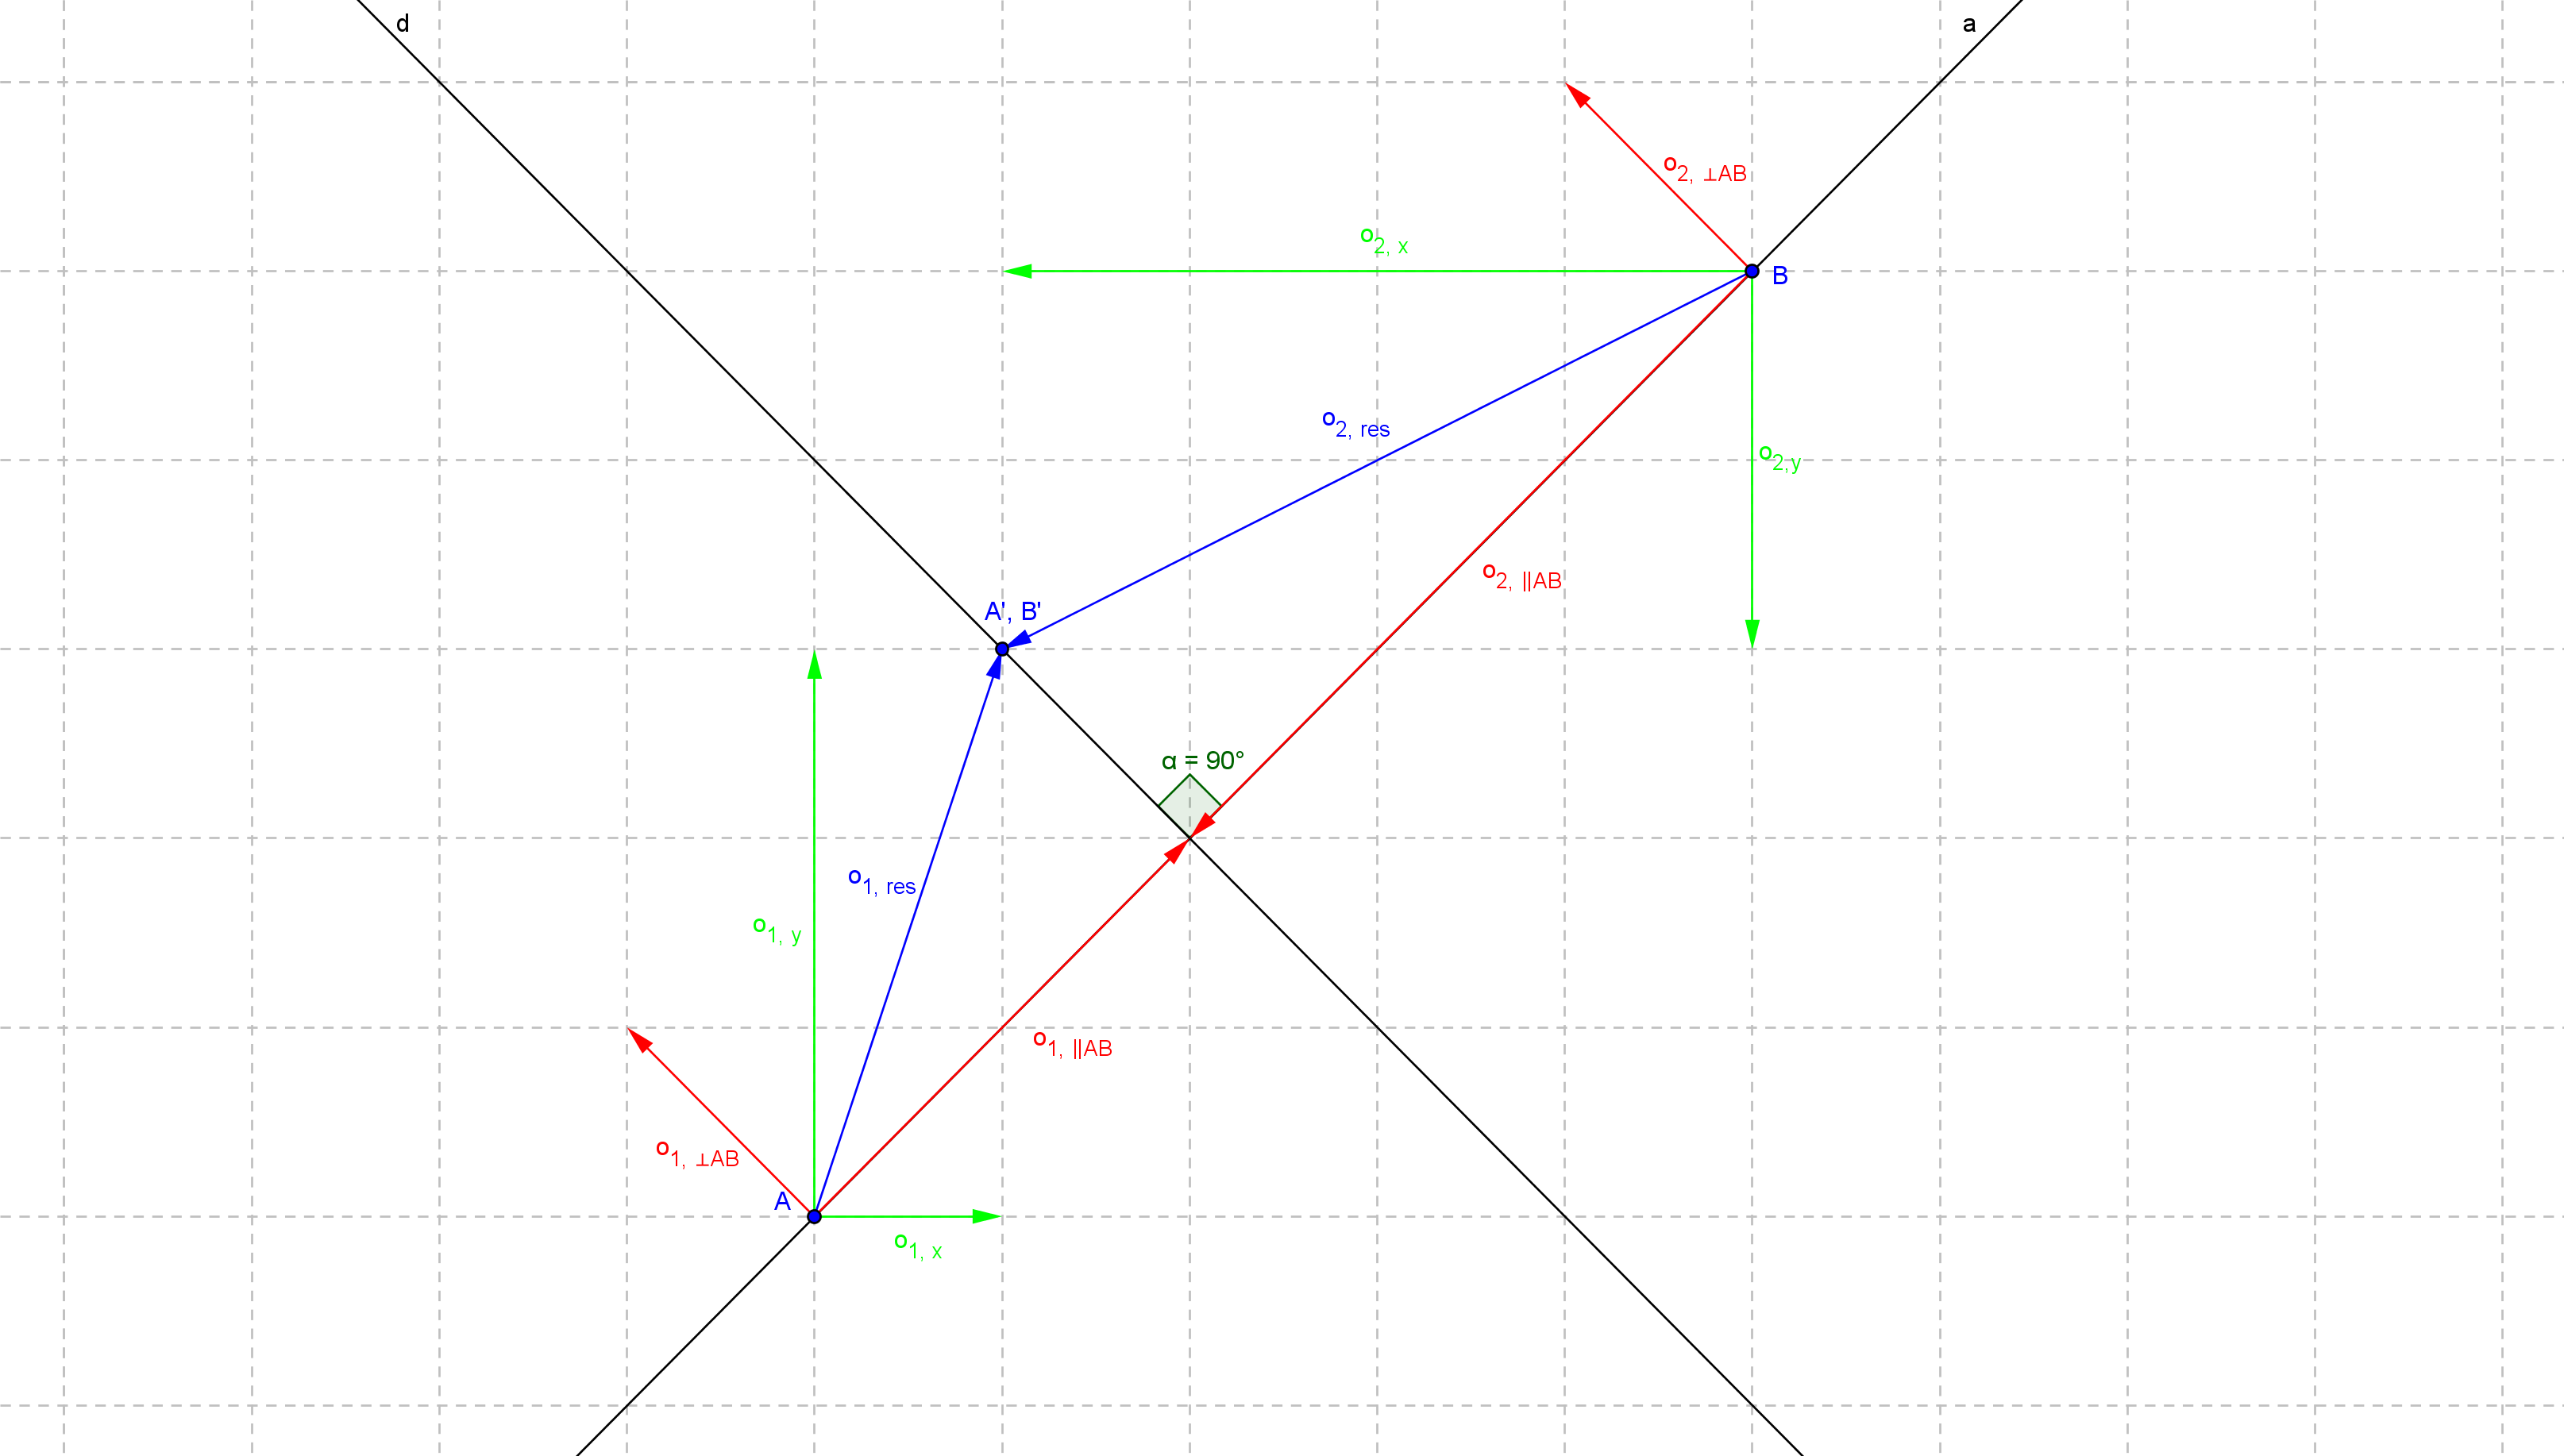
\includegraphics[width=\textwidth]{niet-centrale botsing.png}}
		\caption{Botsing tussen twee ballen}
		\label{niet-centrale botsing}
	\end{figure}
	De snelheden van lichaam 1 en 2  in de richting van de voortplantingsbeweging zijn:
	\begin{equation}
		\begin{aligned}
			o_1=\sqrt{{o_{1,x}}^2+{{o_{1,y}}^2}}\\
			o_2=\sqrt{{o_{2,x}}^2+{{o_{2,y}}^2}}\\
		\end{aligned}
	\end{equation}

	Als we eerst de vergelijking opstellen voor bal 1, zijn die van bal 2 daar eenvoudig uit te herleiden. De positie van bal 1 is $(x_1,y_1)$. Na $\text{1 }s$ is de positie van bal 1 $(x_1+o_{1,x},y_1+o_{1,y})$. Wanneer een frame een andere lengte heeft dan $\text{1 }s$ moeten de snelheden nog vermenigvuldigd worden met een constante. Voor het gemak geven we de verschillende grootheden een letter:
	\begin{equation}
		\begin{aligned}
			A&=\text{lichaam 1}\\
			B&=\text{lichaam 2}\\
			A'&=\text{lichaam 1 op de positie van de botsing}\\
			B'&=\text{lichaam 2 op de positie van de botsing}\\
			a&={x_1}\\
			b&={y_1}\\
			c&={x_2}\\
			d&={y_2}\\
			e&={x_1+o_{1,x}}={x_2+o_{2,x}}\\
			f&={y_1+o_{1,y}}={y_2+o_{2,y}}\\
		\end{aligned}
	\end{equation}
We bekijken de tweedimentionale botsing in het $Oxy$-vlak, en lossen het dan analytisch op. Het middelpunt is $M(\frac{x_1+x_2}{2}, \frac{y_1+y_2}{2})$. De vergelijking voor AM en A'M zijn dan als volgt:

	\begin{equation}
		\begin{aligned}
			AM=AB&: y-b=\frac{b-d}{a-c}\left(x-a\right)\\
			A'M&: y-f=\frac{c-a}{b-d}\left(x-e\right)\\
		\end{aligned}
	\end{equation}

We kunnen het snijpunt van deze twee vergelijkingen berekenen. De $x$-co"{o}rdinaat stelt de snelheid in de $x$-richting naar B voor. De $y$-co\"{o}rdinaat stelt de snelheid in de $y$-richting naar B voor.
	\begin{equation}
		\begin{aligned}
			\frac{b-d}{a-c}\left(x-a\right)+b=&\frac{c-a}{b-d}\left(x-e\right)+f\\
			\left(\frac{b-d}{a-c}+\frac{a-c}{b-d}\right)x=&\frac{b-d}{a-c}a+\frac{a-c}{b-d}e+f-b\\
			\frac{(b-d)^2+(a-c)^2}{(a-c)(b-d)}x=&\frac{a(b-d)^2+e(a-c)^2+(f-b)(a-c)(b-d)}{(a-c)(b-d)}\\
			\left((b-d)^2+(a-c)^2\right)x=&a(b-d)^2+e(a-c)^2+(f-b)(a-c)(b-d)\\
			x=&\frac{a(b-d)^2+e(a-c)^2+(f-b)(a-c)(b-d)}{(b-d)^2+(a-c)^2}\\
		\end{aligned}
	\end{equation}

Invullen in AB geeft 
	\begin{equation}
		\begin{aligned}
			y=\frac{b-d}{a-c}\left(\frac{a(b-d)^2+e(a-c)^2+(f-b)(a-c)(b-d)}{(b-d)^2+(a-c)^2}-a\right)+b\\
		\end{aligned}
	\end{equation}

De snelheid richting B is dus: $o_{1, ||AB}=\sqrt{x^2+y^2}$. Hiervoor geldt dus wel de wet van behoud van impuls. Voor de snelheid loodrecht op de verplaatsingsrichting geldt: $o_{1, LAB}=v_{1, LAB}=\sqrt{{o_{1, res}}^2-{o_{1, ||AB}}^2}$.

De resulterende snelheid na de botsing is: $v_{1, res}=\sqrt{{v_{1, ||AB}}^2+{v_{1, LAB}}^2}$.

De snelheden in de $x$- en $y$-richting kunnen als volgt berekend worden:
	\begin{equation}
		\begin{aligned}
			v_{1, x}=\frac{v_{1, ||AB}\left(a-c\right)+v_{1, LAB}\left(b-d\right)}{\sqrt{\left(a-c\right)^2+\left(b-d\right)^2}}\\
			v_{1, y}=\frac{v_{1, ||AB}\left(b-d\right)+v_{1, LAB}\left(a-c\right)}{\sqrt{\left(a-c\right)^2+\left(b-d\right)^2}}\\
		\end{aligned}
	\end{equation}

Nu $a$, $b$, $c$ en $d$ vervangen door de co\"{o}dinaten:
	\begin{equation}
		\begin{aligned}
			v_{1, x}=\frac{v_{1, ||AB}\left(x_1-x_2\right)+v_{1, LAB}\left(y_1-y_2\right)}{\sqrt{\left(x_1-x_2\right)^2+\left(y_1-y_2\right)^2}}\\
			v_{1, y}=\frac{v_{1, ||AB}\left(y_1-y_2\right)+v_{1, LAB}\left(x_1-x_2\right)}{\sqrt{\left(x_1-x_2\right)^2+\left(y_1-y_2\right)^2}}\\
		\end{aligned}
	\end{equation}

	\newpage
Met alle bekende variabelen:
De resulterende snelheid na de botsing is: 
	\begin{equation}
		\begin{aligned}
			v_{1, res}&=\sqrt{{v_{1, ||AB}}^2+{v_{1, LAB}}^2}\\
			v_{1, res}&=\sqrt{{v_{1, ||AB}}^2+|{o_{1, res}}^2-{o_{1, ||AB}}^2|}\\
			v_{1, res}&=\sqrt{\frac{\left(m_1o_{1, ||AB}+m_2o_{2, ||AB}\right)+m_2\left(o_{2, ||AB}-o_{1, ||AB}\right)}{m_1+m_2}+|{o_{1, res}}^2-{o_{1, ||AB}}^2|}\\
		\end{aligned}
	\end{equation}

	\newpage

	\section{Experiment van botsende ballen}

	\subsection{Verwachtingen bij het experiment van botsende ballen}
	Wij werken alleen met botsingen in het platte vlak. Omdat we werken met harde houten ballen, die vergelijkbaar zijn met biljartballen, hebben we enkel en alleen te maken met volkomen elastische botsingen.

	\subsubsection{Botsing tussen twee ballen}
	Er zijn twee soorten botsingen te onderscheiden: een centrale botsing en een niet-centrale botsing.
De verwachting bij een centrale botsing is, dat de richting van de snelheid van de ballen na de botsing precies tegenovergesteld is aan de richting van de snelheid van de ballen voor de botsing, en dat de snelheden van de ballen verwisseld zijn.
De verwachting bij een niet-centrale botsing waarvan \'{e}\'{e}n bal geen snelheid heeft is, dat de ballen onder een hoek van 90° uitelkaar gaan na de botsing, als de massa's gelijk zijn. 

\begin{figure}[h]
	\centerline{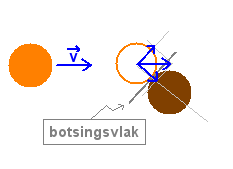
\includegraphics{BotsingSchuin.png}}
	\caption{Een niet-centrale botsing}
	\label{botsingschuin}
\end{figure}

Op deze twee afbeeldingen heeft bal 2 aanvankelijk geen snelheid. Na de botsing zal een deel van de snelheid van bal 1\ ``overgedragen" zijn aan bal 2, en gaan de ballen onder een hoek van 90° uit elkaar.

	Dit is ook als volgt te bewijzen:
	De twee ballen zijn te beschouwen als puntmassa's. We kiezen een assenstelsel zo dat er voor de botsing geen beweging in de $y$-richting is. Bal 1 gaat daarna omhoog onder een hoek $\alpha$ en bal 2 onder een hoek $\beta$. Nu hebben we de volgende gegevens:
	\begin{equation}
	\begin{aligned}
		o_{1, x}&=o_1\\
		o_{1, y}&=0\\
		o_{2, x}&=0\\
		o_{2, y}&=0\\
	\end{aligned}
	\end{equation}

	Volgens de wet van behoud van impuls geldt voor de $x$-richting:
	\begin{equation}
	\begin{aligned}
	\label{voorbeeld 1.1}
		mo_{1, x}&=mv_{1, x}+mv_{2, x}\\
		mo_{1, x}&=mv_1cos(\alpha)+mv_2cos(\beta)\\
		{o_{1, x}}^2&={v_1}^2cos^2(\alpha)+{v_2}^2cos^2(\beta)+2v_1v_2cos(\alpha)cos(\beta)\\
	\end{aligned}
	\end{equation}

	En in de $y$-richting geldt:
	\begin{equation}
	\begin{aligned}
	\label{voorbeeld 1.2}
		mo_{1, y}&=mv_{1, y}+mv_{2, y}\\
		0&=mv_{1, y}+mv_{2, y}\\
		0&=mv_1sin(\alpha)+mv_2sin(\beta)\\
	\end{aligned}
	\end{equation}

	Ook geldt de wet van behoud van energie:
	\begin{equation}
	\begin{aligned}
	\label{voorbeeld 1.3}
		m{o_1}^2&=m{v_1}^2+m{v_2}^2\\
		{o_1}^2&={v_1}^2+{v_2}^2\\
	\end{aligned}
	\end{equation}

	Met $sin^2(\alpha)+cos^2(\alpha)=1$ en invullen van \eqref{voorbeeld 1.1} en \eqref{voorbeeld 1.3} in elkaar, levert dat op:
	\begin{equation}
	\begin{aligned}
	\label{voorbeeld 1.4}
		2v_1v_2cos(\alpha)cos(\beta)&={v_1}^2sin^2(\alpha)+{v_2}^2sin^2{\beta}\\
	\end{aligned}
	\end{equation}

	Met gebruik van \eqref{voorbeeld 1.2} in \eqref{voorbeeld 1.4} krijg je dan:
	\begin{equation}
	\begin{aligned}
	\label{voorbeeld 1.5}
		2v_1v_2cos(\alpha)cos(\beta)&=2v_1v_2sin(\alpha)sin(\beta)\\
	\end{aligned}
	\end{equation}

	Dit levert op $tan(\alpha)tan(\beta)=1$ waardoor de hoek $\alpha+\beta=90°$.

	\subsubsection{Botsing tussen meer dan twee ballen}
	In de werkelijkheid zal het nauwelijks voorkomen dat een botsing tussen meer dan twee ballen plaatsvindt. Als dit wel zo lijkt zijn het meestal meerdere botsingen vlak na elkaar. Maar in theorie is het best mogelijk dat drie ballen elkaar exact op hetzelfde ogenblik raken. Wij verwachten dat deze botsing te schrijven is als de som van twee botsingen tussen twee ballen.
Het maximale aantal ballen, dat elkaar tegelijk in het platte vlak kunnen raken is drie. Het maximale aantal ballen, dat een andere bal tegelijkertijd kunnen raken is zes. Als drie ballen elkaar kunnen raken, is de hoek bal bal bal 60°. Er kunnen dus 360°/60° = 6 ballen om een andere bal heen liggen. Waarschijnlijk zijn deze botsingen te schrijven is als de som van meerdere botsingen tussen twee ballen.

	\subsection{Resultaten van het experiment met botsende ballen}
	Om te controleren of de formules - die afgeleidt zijn van de wet van behoud van impuls - ook in overeenstemming zijn met de werkelijkheid, hebben wij een aantal proeven uitgevoerd. We hebben de proeven uitgevoerd op 15 december 2010 in het practicumlokaal, meer een camera van school. Deze proeven hebben we uitgevoerd met verschillende ballen, omdat we van tevoren niet wisten bij welke ballen de meeste kinetische energie werd overgedragen. We hebben een golfbal, knikkers en jeu de boules ballen gebruikt. Eerst wilden we een aantal gegevens noteren van de ballen die wij gebruikten, zoals de diameter of omtrek en de massa. Maar we omdat alleen de massa's en de snelheden van de ballen in de formules \eqref{energie} en \eqref{impuls} hebben zitten, hebben we alleen de massa's van de ballen genoteerd:

	\begin{tabular}{|  l l |}
		\hline 
			\emph{lichaam} &\emph{massa}\\
			Golfbal: &045,98 gram\\
			Gele knikker: &104,42 gram\\
			Witte knikker: &089,75 gram\\
			Zwart-witte knikker: &091,27 gram\\
			Groene jeu de boules bal: &228,04 gram\\
			Blauwe jeu de boules bal: &223,06 gram\\
			Rode jeu de boules bal: &223,30 gram\\
		\hline 
	\end{tabular}
	\\
	\\We hebben een aantal verschillende combinaties van ballen met elkaar laten botsen. Eerst een blauwe jeu de boules bal met een rode jeu de boules bal.

In figuur \eqref{botsing3} zijn alle beeldjes van de botsing samengevoegd, zodat de botsing duidelijk te zien is.

\begin{figure}[h]
	\centerline{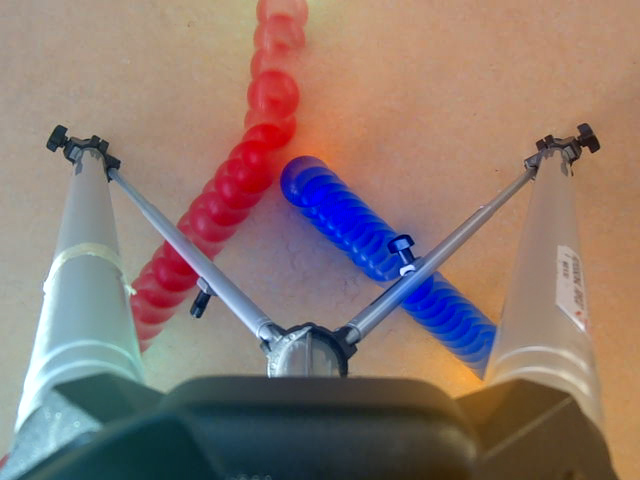
\includegraphics[width=0.5\textwidth]{botsing3.jpg}}
	\caption{Alle beeldjes samengevoegd}
	\label{botsing3}
\end{figure}

	Als we de resultaten met Coach uitlezen en in tabellen zetten, kunnen we er met Exel hieraan rekenen. Als we de positie uitzetten tegen de tijd krijgen we figuur \eqref{00771} en \eqref{00772}.

\begin{figure}[h]
	\centerline{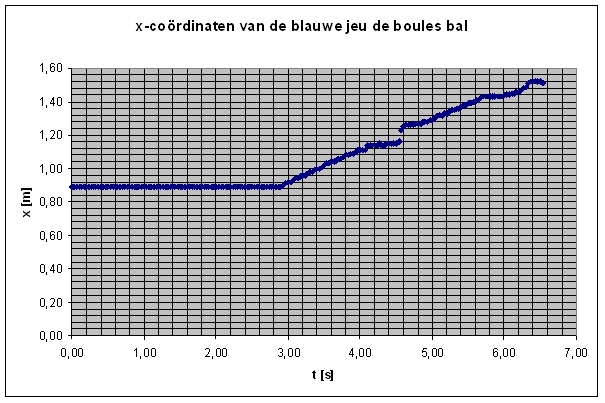
\includegraphics[width=0.5\textwidth]{00771.png}}
	\caption{x-co\"{o}rdinaten van de blauwe jeu de boules bal}
	\label{00771}
\end{figure}

\begin{figure}[h]
	\centerline{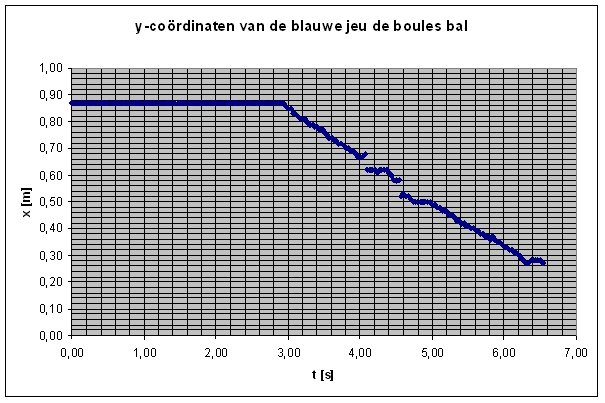
\includegraphics[width=0.5\textwidth]{00772.png}}
	\caption{y-co\"{o}rdinaten van de blauwe jeu de boules bal}
	\label{00772}
\end{figure}

	De blauwe bal licht in eerste instantie stil. Pas vanaf $t=2,94\ s$ begint de blauwe bal te rollen, nadat de rode bal er tegen aan is gebotst. Op ongeveer $t=4,30\ s$ tot $t=4,54\ s$ rolt de blauwe bal onder de paal door, hierdoor is het automatisch traceren op dit interval niet goed gelukt. Na $t=5,71\ s$ verdwijnt de bal uit het beeld, en is dus ook niet goed getraceerd. Als we dus alleen de goede meetresultaten mee rekenen krijgen we reeks \eqref{00773} en \eqref{00774}.

\begin{figure}[h]
	\centerline{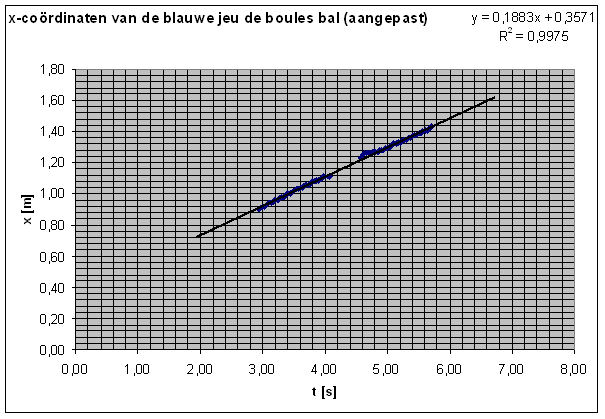
\includegraphics[width=0.5\textwidth]{00773.png}}
	\caption{x-co\"{o}rdinaten van de blauwe jeu de boules bal (aangepast)}
	\label{00773}
\end{figure}

\begin{figure}[h]
	\centerline{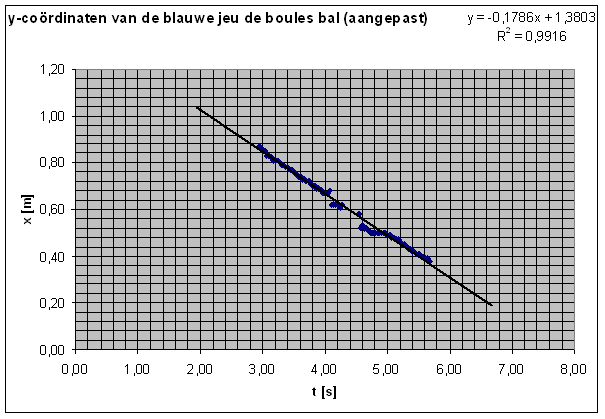
\includegraphics[width=0.5\textwidth]{00774.png}}
	\caption{y-co\"{o}rdinaten van de blauwe jeu de boules bal (aangepast)}
	\label{00774}
\end{figure}

	Nu hebben we de plaats in de $x$-richting en in de $y$-richting uitgezet tegen de tijd. Hieruit kunnen we de snelheid van de bal herleiden. Na $1,00\ s$ is de bal $0,1883\ m$ verplaats in de $x$-richting en $0,1786\ m$ in de $y$-richting. De snelheid van de bal kun je dus berekenen met de $Stelling\ van\ Pythagoras$:

	\begin{equation}
		\label{snelheid}
		\begin{aligned}
			v&=\sqrt{{|rc_x|}^2+{|rc_y|}^2}\\
			v&=\sqrt{{rc_x}^2+{rc_y}^2}\\
		\end{aligned}
	\end{equation}

	De snelheid van de blauwe jeu de boules bal na de botsing is dus: $v=\sqrt{{0,1883}^2+{0,1786}^2}=0,2595\ m/s$

	Nu hebben we de blauwe bal gehad, nu de rode bal. De rode bal heeft, in tegenstelling tot de blauwe, wel een begin snelheid. Omdat de rode bal heel weinig wordt afgebogen is het niet heel duidelijk te zien op werk tijdstip dit gebeurd. De bal wordt het meeste afgebogen in de $x$-richting, en als we in figuur \eqref{00775} kijken kunnen we op $t=2,97\ s$ een verandering in de baan ontdekken.

\begin{figure}[h]
	\centerline{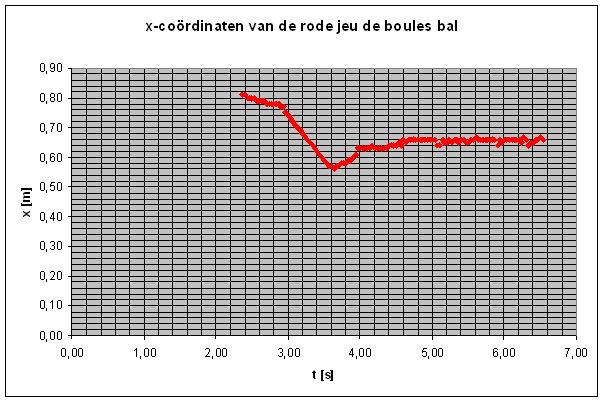
\includegraphics[width=0.5\textwidth]{00775.png}}
	\caption{x-co\"{o}rdinaten van de rode jeu de boules bal}
	\label{00775}
\end{figure}

\begin{figure}[h]
	\centerline{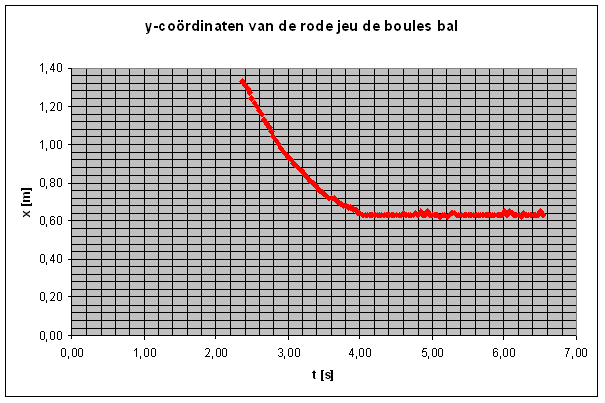
\includegraphics[width=0.5\textwidth]{00776.png}}
	\caption{y-co\"{o}rdinaten van de rode jeu de boules bal}
	\label{00776}
\end{figure}

De punten van figuur \eqref{00777} lijken een beetje vreemd, maar dat komt omdat we maar een klein aantal beeldjes hebben van de rode bal voor de botsing, de bal nauwelijk zich in de $x$-richting verplaatst en omdat het traceren niet nauwkeuriger gebeurt dan met twee decimalen.

\begin{figure}[h]
	\centerline{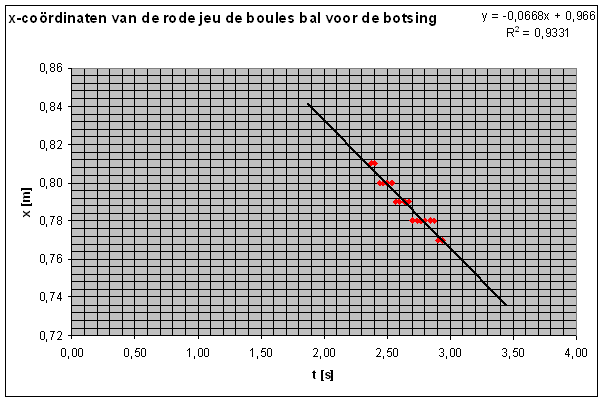
\includegraphics[width=0.5\textwidth]{00777.png}}
	\caption{x-co\"{o}rdinaten van de rode jeu de boules bal voor de botsing}
	\label{00777}
\end{figure}

\begin{figure}[h]
	\centerline{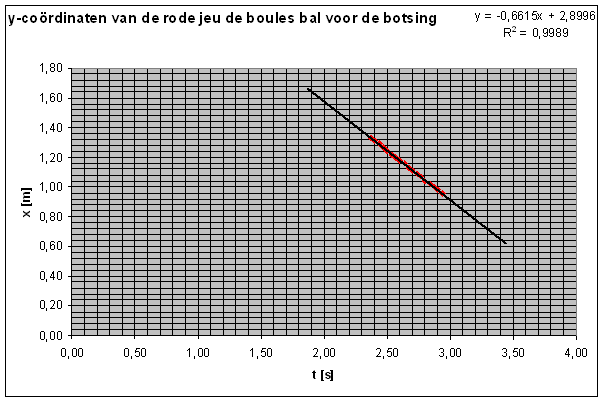
\includegraphics[width=0.5\textwidth]{00778.png}}
	\caption{y-co\"{o}rdinaten van de rode jeu de boules bal voor de botsing}
	\label{00778}
\end{figure}

Hier doen we dus hetzelfde mee als met de blauwe jeu de boules bal. De snelheid berekenen we dus met formule \eqref{snelheid}: $v=0,6649m/s$

We hebben nu alleen nog maar de snelheid van de rode bal na de botsing nodig. Op figuur \eqref{00775} is te zien dat de bal op $t=3,67\ s$ onder de paal door gaat en het traceren niet meer wil. Als we dus de meetresultaten van $t=2,79\ s$ tot $t=3,67\ s$ nemen krijgen we figuur \eqref{00779} en \eqref{007710}.

\begin{figure}[h]
	\centerline{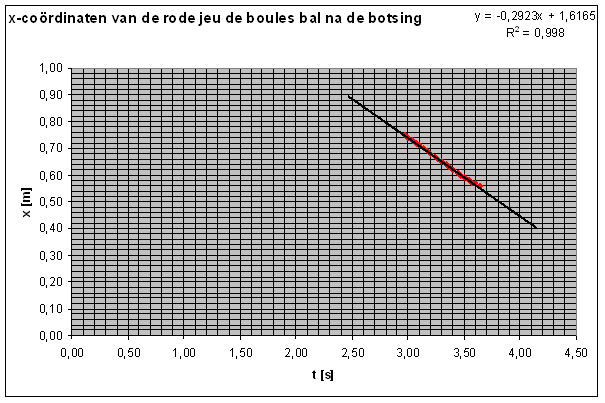
\includegraphics[width=0.5\textwidth]{00779.png}}
	\caption{$x$-co\"{o}rdinaten van de rode jeu de boules bal na de botsing}
	\label{00779}
\end{figure}

\begin{figure}[h]
	\centerline{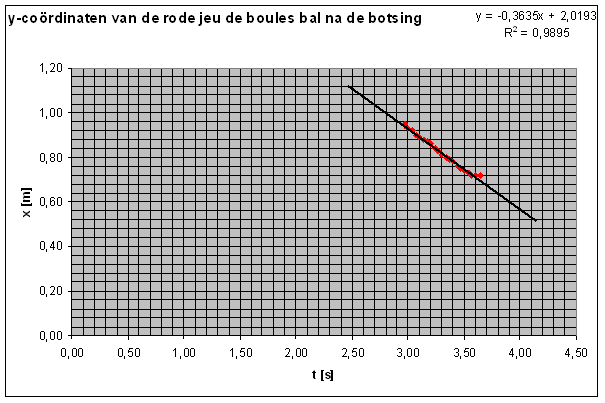
\includegraphics[width=0.5\textwidth]{007710.png}}
	\caption{$y$-co\"{o}rdinaten van de rode jeu de boules bal na de botsing}
	\label{007710}
\end{figure}

	De snelheid hieruit berekenen geeft: $v=0,4664m/s$

	We stellen dat de blauwe bal, bal 1 is, en de rode bal, bal 2.
	Dan hadden we de volgende gegevens:

	\begin{tabular}{  l l }
		$m_1$= &0,22306 kg\\
		$m_2$= &0,22330 kg\\
		$o_1$= &0,0000 m/s\\
		$o_2$= &0,6649 m/s\\
	\end{tabular}

	Als het een centrale botsing zou zijn, dan zouden de snelheden na de botsing berekend kunnen worden met de formules van \eqref{uitwerking-energie-impuls}.
	$v_1$ zou in dat geval moeten zijn:

	\begin{equation}
		\begin{aligned}
			v_1&=\frac{\left(0,22306 \cdot 0,0000+0,22330 \cdot 0,6649\right)+0,22330 \cdot \left(0,6649-0,0000\right)}{\left(0,22306+0,22330\right)}=0,6653m/s\\
		\end{aligned}
	\end{equation}

	En $v_2$ zou moeten zijn:

	\begin{equation}
		\begin{aligned}
			v_2&=\frac{\left(0,22330 \cdot 0,6649+0,22306 \cdot 0,0000\right)+0,22306 \cdot \left(0,0000-0,6649\right)}{\left(0,22330+0,22306\right)}=0m/s
		\end{aligned}
	\end{equation}

Maar in dit geval hebben we te maken met een niet-centrale botsing.

	\newpage

	\section{Programmeren}
	\subsection{Andere eenheden}
	Een computermodel gebruikt andere eenheden dan in de realiteit worden gebruikt, dus we defini\"{e}ren hier nieuwe eenheden. Als eerste werkt een animatie met een hoeveelheid beeldjes per seconde, of in het Engels: \emph{frames per seconde} (fps). We proberen een snelheid van ongeveer $80$fps te bereiken; hoe hoger het aantal frames per seconde, hoe betrouwbaarder de simulatie. De snelheid van de voorwerpen geven we vervolgens in pixels per frame, of het aantal beeldpuntjes per frame. Dus komen we tot de volgende definities:
	\\
	\begin{tabular}{| l l l l |}
		\hline 
		\emph{grootheid}       & \emph{symbool} & \emph{eenheid}                    & \emph{symbool} \\
		Interval tussen frames & $T$            & seconden                          & $s$            \\
		Frames per seconde     & $f$            & hertz                             & Hz = $s^{-1}$  \\
		Snelheid               & $v$            & pixels per interval               & px T$^{-1}$    \\
		Versnelling            & $a$            & pixels per intervalkwadraat       & px T$^{-2}$    \\
		Kracht                 & $F$            & newton.... .hoehierverder.        & $?$            \\
		\hline 
	\end{tabular}
	
	\subsection{Hoe de posities berekend worden}
	In onze simulatie nemen we steeds een stapje $T$ verder in de tijd. Elke keer als we een stapje verder gaan doen we de volgende stappen:
	\\
	\begin{enumerate}[1]
		\item Ga alle voorwerpen bij langs
		\begin{enumerate}[1]
			\item Bereken de nieuwe positie: Tel de snelheidsvector bij de huidige positie op
			\item Bereken welke de richting en grootte van alle krachten op het voorwerp
			\item Bereken met behulp van de som van alle krachten de nieuwe versnelling
			\item Tel de versnelling bij de snelheid op
		\end{enumerate}
	\end{enumerate}
	We doen dus alsof elk voorwerp met een constante snelheid in het interval $T$ beweegt. Dit klopt niet met de realiteit, maar als we het tijdsinterval tussen twee frames steeds kleiner maken, benadert het wel de werkelijkheid. Stel dat $T$ naar 0 nadert, dus $T = \Delta t$, dan geldt allereerst voor de positie van een voowerp:
	\\	
	\begin{equation}
		\label{verplaatsing}
		\begin{aligned}
			\mathbf{x} =: \mathbf{x} + \mathbf{v} \cdot \Delta t
		\end{aligned}	
	\end{equation}
	En voor de snelheid geldt dan:
	\\	
	\begin{equation}
		\label{snelheidsdefinitie}
		\begin{aligned}
			\mathbf{v} &= \lim_{\Delta t\to0} \frac{\Delta \mathbf{x}}{\Delta t} \\
			\mathbf{v} \cdot \Delta t &= \Delta \mathbf{x}
		\end{aligned}
	\end{equation}
	Invullen van \eqref{snelheidsdefinitie} in \eqref{verplaatsing} geeft dan:
	\begin{equation}
		\mathbf{x} =: \mathbf{x} +  \Delta \mathbf{x}
	\end{equation}
	Waarmee bewezen is dat je de snelheid van een voorwerp als constant mag zien in een minuscuul tijdsinterval.
\end{document}

	\newpage

	\section{Conclusie}



